% Options for packages loaded elsewhere
\PassOptionsToPackage{unicode}{hyperref}
\PassOptionsToPackage{hyphens}{url}
%
\documentclass[
]{article}
\usepackage{amsmath,amssymb}
\usepackage{lmodern}
\usepackage{iftex}
\usepackage[margin=0.5in]{geometry}
\ifPDFTeX
  \usepackage[T1]{fontenc}
  \usepackage[utf8]{inputenc}
  \usepackage{textcomp} % provide euro and other symbols
\else % if luatex or xetex
  \usepackage{unicode-math}
  \defaultfontfeatures{Scale=MatchLowercase}
  \defaultfontfeatures[\rmfamily]{Ligatures=TeX,Scale=1}
\fi
% Use upquote if available, for straight quotes in verbatim environments
\IfFileExists{upquote.sty}{\usepackage{upquote}}{}
\IfFileExists{microtype.sty}{% use microtype if available
  \usepackage[]{microtype}
  \UseMicrotypeSet[protrusion]{basicmath} % disable protrusion for tt fonts
}{}
\makeatletter
\@ifundefined{KOMAClassName}{% if non-KOMA class
  \IfFileExists{parskip.sty}{%
    \usepackage{parskip}
  }{% else
    \setlength{\parindent}{0pt}
    \setlength{\parskip}{6pt plus 2pt minus 1pt}}
}{% if KOMA class
  \KOMAoptions{parskip=half}}
\makeatother
\usepackage{xcolor}
\IfFileExists{xurl.sty}{\usepackage{xurl}}{} % add URL line breaks if available
\IfFileExists{bookmark.sty}{\usepackage{bookmark}}{\usepackage{hyperref}}
\hypersetup{
  pdftitle={087hw9},
  hidelinks,
  pdfcreator={LaTeX via pandoc}}
\urlstyle{same} % disable monospaced font for URLs
\usepackage{graphicx}
\makeatletter
\def\maxwidth{\ifdim\Gin@nat@width>\linewidth\linewidth\else\Gin@nat@width\fi}
\def\maxheight{\ifdim\Gin@nat@height>\textheight\textheight\else\Gin@nat@height\fi}
\makeatother
% Scale images if necessary, so that they will not overflow the page
% margins by default, and it is still possible to overwrite the defaults
% using explicit options in \includegraphics[width, height, ...]{}
\setkeys{Gin}{width=\maxwidth,height=\maxheight,keepaspectratio}
% Set default figure placement to htbp
\makeatletter
\def\fps@figure{htbp}
\makeatother
\setlength{\emergencystretch}{3em} % prevent overfull lines
\providecommand{\tightlist}{%
  \setlength{\itemsep}{0pt}\setlength{\parskip}{0pt}}
\setcounter{secnumdepth}{-\maxdimen} % remove section numbering
\ifLuaTeX
  \usepackage{selnolig}  % disable illegal ligatures
\fi

\usepackage{fancyvrb}

\begin{document}

\noindent Nathan Burwig \\
Math 87 HW 7 \\
Due 11/12/2022
    
\hrulefill

What follows is the complete output of my jupyter notebook file, formatted to
make it a decent big more readable. At the end, I will answer all of the
questions individually, though I believe most of the questions are answered
throughout the notebook.

\hypertarget{Is-it-a-hot-dogux2c-or-not-ux28dogux29ux3f}{%
\section{\texorpdfstring{Is it a hot dog, or not
(dog)?\protect\hyperlink{Is-it-a-hot-dogux2c-or-not-ux28dogux29ux3f}{¶}}{Is it a hot dog, or not (dog)?¶}}\label{Is-it-a-hot-dogux2c-or-not-ux28dogux29ux3f}}

This is an attempt at classifying a set of images as either hot dogs or
not hot dogs. I'll be using tensorflow, and a hotdog image set with
training data found online.


\begin{Verbatim}[frame=single]
import os
from os.path import join
import tensorflow as tf
import matplotlib.pyplot as plt
from IPython.display import Image, display
import numpy as np
from tensorflow.keras.applications.resnet50 import preprocess_input
from tensorflow.keras.applications import ResNet50
from tensorflow.keras.preprocessing.image import load_img, img_to_array
\end{Verbatim}


\begin{Verbatim}[frame=single]
print("TensorFlow version:", tf.__version__)
\end{Verbatim}

\begin{verbatim}
TensorFlow version: 2.11.0
\end{verbatim}


\begin{Verbatim}[frame=single]
image_size = 224

## imports images and outputs an array
def prep_images(img_paths, img_height=image_size, img_width=image_size):
    ## loading images in the image paths
    imgs = [load_img(img_path, target_size=(img_height, img_width)) for img_path in img_paths]


    ## converting images to arrays and returning
    img_array = np.array([img_to_array(img) for img in imgs])
    output = preprocess_input(img_array)
    print(np.shape(imgs[0]))
    print(np.shape(img_array[0]))
    return (output)
\end{Verbatim}

We can now get the training data, they will be in categories either "hot
dog" or "not hot dog"

\begin{Verbatim}[frame=single]
train_hotdog_dir    = 'C:\\Users\\nburw\\OneDrive\\Desktop\\train\\hot_dog'
train_nothotdog_dir = 'C:\\Users\\nburw\\OneDrive\\Desktop\\train\\not_hot_dog'
\end{Verbatim}

Quick test to make sure directories are okay

\begin{Verbatim}[frame=single]
print(train_hotdog_dir)
print(train_nothotdog_dir)
\end{Verbatim}

\begin{verbatim}
C:\Users\nburw\OneDrive\Desktop\train\hot_dog
C:\Users\nburw\OneDrive\Desktop\train\not_hot_dog
\end{verbatim}

\begin{Verbatim}[frame=single]
train_hotdog_filenames      = os.listdir(train_hotdog_dir)
train_nothotdog_filenames   = os.listdir(train_nothotdog_dir)
\end{Verbatim}

\newpage
\begin{Verbatim}[frame=single]
hotdog_paths       = [(train_hotdog_dir    + '\\' + train_hotdog_filenames[i])    
                      for i in range(len(train_hotdog_filenames))]
nothotdog_paths    = [(train_nothotdog_dir + '\\' + train_nothotdog_filenames[i]) 
                      for i in range(len(train_nothotdog_filenames))]
\end{Verbatim}

Cool, so now we have a way to get paths for individual images, so we can
start getting tensorflow out now. That was a bit of a lie, but first we
need to get the training set setup. Training sets are gonna be an array
of x,y pairs where x is an image (as an array) and y is a value from 0
to 1 where 1 means it's a hot dog, and 0 means it's not a hot dog.

\begin{Verbatim}[frame=single]
prepped_hotdogs     = prep_images(hotdog_paths)
prepped_nothotdogs  = prep_images(nothotdog_paths)
\end{Verbatim}

Now we convert into the xy pair

\begin{Verbatim}[frame=single]
x_train = np.concatenate((prepped_hotdogs, prepped_nothotdogs))
y_train = np.array([(1 if n <= 249 else 0) for n in range(len(x_train))])

print(np.shape(x_train), np.shape(y_train))
\end{Verbatim}

\begin{verbatim}
(498, 224, 224, 3) (498,)
\end{verbatim}

\begin{Verbatim}[frame=single]
## now we shuffle them in unison
assert len(x_train) == len(y_train)

##    Example    ##
a = np.array([1, 2, 3, 4, 5])
b = np.array([-1, -2, -3, -4, -5])

p = np.random.permutation(len(a))
print(a[p])
print(b[p])
## Example (end) ##

## actual unison shuffle of data
shuffler = np.random.permutation(len(x_train))
y_train = y_train[shuffler]
x_train = x_train[shuffler]
\end{Verbatim}

\begin{verbatim}
[4 1 5 2 3]
[-4 -1 -5 -2 -3]
\end{verbatim}


\begin{Verbatim}[frame=single]
import matplotlib.pyplot as plt
plt.imshow(prepped_hotdogs[1])
print(np.shape(prepped_hotdogs[0]))
\end{Verbatim}

\begin{verbatim}
Clipping input data to the valid range for imshow with RGB data ([0..1] for floats or [0..255] for integers).
\end{verbatim}

\begin{verbatim}
(224, 224, 3)
\end{verbatim}

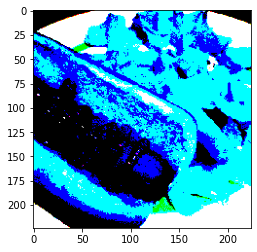
\includegraphics{bef603d52cf14721fe48e3182b104cf14476e163.png}

Okay so now we have our training data setup. We are going to setup our
model using tf.keras now.

\hypertarget{Developing-Models}{%
\section{\texorpdfstring{Developing
Models\protect\hyperlink{Developing-Models}{¶}}{Developing Models¶}}\label{Developing-Models}}

For our first attempt, we will be using a convolutional network

\begin{Verbatim}[frame=single]
model_v1 = tf.keras.models.Sequential([
    tf.keras.layers.Conv2D(16, kernel_size=(3,3), activation='relu', input_shape=(224,224,3)),
    tf.keras.layers.Conv2D(32, kernel_size=(3,3), activation='relu'),
    tf.keras.layers.Flatten(),
    tf.keras.layers.Dropout(0.2),
    tf.keras.layers.Dense(2)
    ])
\end{Verbatim}

Here we define a loss function

\begin{Verbatim}[frame=single]
loss_fn = tf.keras.losses.SparseCategoricalCrossentropy(from_logits=True)
\end{Verbatim}

\begin{Verbatim}[frame=single]
predictions = model_v1(x_train[:1]).numpy()
print(predictions)
\end{Verbatim}

\begin{verbatim}
[[-12.270783   -7.8165493]]
\end{verbatim}

\begin{Verbatim}[frame=single]
tf.nn.softmax(predictions).numpy()
\end{Verbatim}

Out{[}~{]}:

\begin{verbatim}
array([[0.01149554, 0.98850447]], dtype=float32)
\end{verbatim}

Does this mean the model is predicting that this image is a hotdog? I
don't completely understand...

Compile the model

\begin{Verbatim}[frame=single]
model_v1.compile(optimizer='adam',
              loss=loss_fn,
              metrics=['accuracy'])
\end{Verbatim}

Time to train

\begin{Verbatim}[frame=single]
model_v1.fit(x_train, y_train, epochs=6)
\end{Verbatim}

\begin{verbatim}
Epoch 1/6
16/16 [==============================] - 33s 2s/step - loss: 2092.5833 - accuracy: 0.5482
Epoch 2/6
16/16 [==============================] - 26s 2s/step - loss: 78.5949 - accuracy: 0.6265
Epoch 3/6
16/16 [==============================] - 28s 2s/step - loss: 6.6297 - accuracy: 0.8112
Epoch 4/6
16/16 [==============================] - 26s 2s/step - loss: 0.8133 - accuracy: 0.9478
Epoch 5/6
16/16 [==============================] - 27s 2s/step - loss: 0.2848 - accuracy: 0.9759
Epoch 6/6
16/16 [==============================] - 28s 2s/step - loss: 0.0389 - accuracy: 0.9940
\end{verbatim}

\begin{verbatim}
<keras.callbacks.History at 0x29fa7008700>
\end{verbatim}

Okay, so now we want to test our data, so we need to create a testing
set. After that, we will evaluate our model, and play around with a few
different model setups to determine the impact on our accuracy.

\hypertarget{Developing-Test-Data}{%
\section{\texorpdfstring{Developing Test
Data\protect\hyperlink{Developing-Test-Data}{¶}}{Developing Test Data¶}}\label{Developing-Test-Data}}

So now we need to go through and develop a test data set. What we are
going to do is grab images from our training data set which contains no
shared images of hotdogs, so the model can't just identify something it
already was trained on. We will quickly run through the same steps we
did in the beginning.

\begin{Verbatim}[frame=single]
test_hotdog_dir    = 'C:\\Users\\nburw\\OneDrive\\Desktop\\test\\hot_dog'
test_nothotdog_dir = 'C:\\Users\\nburw\\OneDrive\\Desktop\\test\\not_hot_dog'

test_hotdog_filenames      = os.listdir(test_hotdog_dir)
test_nothotdog_filenames   = os.listdir(test_nothotdog_dir)

hotdog_paths_test       = [(test_hotdog_dir    + '\\' + test_hotdog_filenames[i])    
                            for i in range(len(test_hotdog_filenames))]
nothotdog_paths_test    = [(test_nothotdog_dir + '\\' + test_nothotdog_filenames[i]) 
                            for i in range(len(test_nothotdog_filenames))]
\end{Verbatim}

\begin{Verbatim}[frame=single]
prepped_hotdogs_test     = prep_images(hotdog_paths_test)
prepped_nothotdogs_test  = prep_images(nothotdog_paths_test)
\end{Verbatim}

\begin{verbatim}
(224, 224, 3)
(224, 224, 3)
(224, 224, 3)
(224, 224, 3)
\end{verbatim}

\begin{Verbatim}[frame=single]
x_test = np.concatenate((prepped_hotdogs_test, prepped_nothotdogs_test))
y_test = np.array([(1 if n <= 249 else 0) for n in range(len(x_test))])

print(np.shape(x_test), np.shape(y_test))
\end{Verbatim}

\begin{verbatim}
(500, 224, 224, 3) (500,)
\end{verbatim}

\begin{Verbatim}[frame=single]
## now we shuffle them in unison
assert len(x_test) == len(y_test)

## actual unison shuffle of data
shuffler = np.random.permutation(len(x_test))
y_test = y_test[shuffler]
x_test = x_test[shuffler]
\end{Verbatim}

\begin{Verbatim}[frame=single]
model_v1.evaluate(x_test,  y_test, verbose=1)
\end{Verbatim}

\begin{verbatim}
16/16 [==============================] - 5s 238ms/step - loss: 12.7981 - accuracy: 0.5040
\end{verbatim}

\begin{verbatim}
[12.79814624786377, 0.5040000081062317]
\end{verbatim}

OK so now that we have a model, and we've tested it (and it frankly
worked out quite poorly) we are gonna start playing around with
different models.

\hypertarget{Playing-with-Different-Models}{%
\section{\texorpdfstring{Playing with Different
Models\protect\hyperlink{Playing-with-Different-Models}{¶}}{Playing with Different Models¶}}\label{Playing-with-Different-Models}}

First and foremost, I'm going to print out the model\_v1 summary so we
know what layers we had originally

\begin{Verbatim}[frame=single]
model_v1.summary()
\end{Verbatim}

\begin{Verbatim}
Model: "sequential_5"
_________________________________________________________________
 Layer (type)                Output Shape              Param #   
=================================================================
 conv2d_6 (Conv2D)           (None, 222, 222, 16)      448       
                                                                 
 conv2d_7 (Conv2D)           (None, 220, 220, 32)      4640      
                                                                 
 flatten_5 (Flatten)         (None, 1548800)           0         
                                                                 
 dropout_5 (Dropout)         (None, 1548800)           0         
                                                                 
 dense_7 (Dense)             (None, 2)                 3097602   
                                                                 
=================================================================
Total params: 3,102,690
Trainable params: 3,102,690
Non-trainable params: 0
_________________________________________________________________
\end{Verbatim}

Immediately I'm curious about what happens if I don't use convolutions,
and instead use a much simpler model. I'll be using just a 4 layer
sequential model to see how it goes. My immediate prediction is that I
will have a worse accuracy, so let's see what happens.

\hypertarget{Model_v2}{%
\subsection{\texorpdfstring{Model\_v2\protect\hyperlink{Model_v2}{¶}}{Model\_v2¶}}\label{Model_v2}}

\begin{Verbatim}[frame=single]
model_v2 = tf.keras.models.Sequential([
  tf.keras.layers.Flatten(input_shape=(224, 224, 3)),
  tf.keras.layers.Dense(128, activation='relu'),
  tf.keras.layers.Dropout(0.2),
  tf.keras.layers.Dense(2)
])

model_v2.compile(optimizer='adam',
              loss=loss_fn,
              metrics=['accuracy'])


model_v2.fit(x_train, y_train, epochs=6)
\end{Verbatim}

\begin{verbatim}
Epoch 1/6
16/16 [==============================] - 4s 223ms/step - loss: 114.7943 - accuracy: 0.8373
Epoch 2/6
16/16 [==============================] - 3s 214ms/step - loss: 237.4119 - accuracy: 0.8373
Epoch 3/6
16/16 [==============================] - 3s 211ms/step - loss: 78.6632 - accuracy: 0.8655
Epoch 4/6
16/16 [==============================] - 3s 215ms/step - loss: 138.4023 - accuracy: 0.8454
Epoch 5/6
16/16 [==============================] - 3s 209ms/step - loss: 45.1477 - accuracy: 0.8976
Epoch 6/6
16/16 [==============================] - 3s 206ms/step - loss: 60.4015 - accuracy: 0.8896
\end{verbatim}

\begin{verbatim}
<keras.callbacks.History at 0x29fa6d1d5b0>
\end{verbatim}

Immediately we can tell this is going worse. I expected we'd need more
epochs to get to a similar level of accuracty for the training data, and
I was right. I don'tknow if adding more is useful becuase it seems to
platue

\begin{Verbatim}[frame=single]
model_v2.evaluate(x_test, y_test, verbose=1)
\end{Verbatim}

\begin{verbatim}
16/16 [==============================] - 1s 20ms/step - loss: 1760.8885 - accuracy: 0.5000
\end{verbatim}

\begin{verbatim}
[1760.8885498046875, 0.5]
\end{verbatim}

Surprisingly close to the original convolutional model... Let's try
another convolutional mode, but which has more dense layers. I'm going
to include a dense layer before the first conv layer to see if that
helps at all.

\hypertarget{Model_v3}{%
\subsection{\texorpdfstring{Model\_v3\protect\hyperlink{Model_v3}{¶}}{Model\_v3¶}}\label{Model_v3}}

\begin{Verbatim}[frame=single]
## Our first attempt will be a generic sequential model with 4 layers
model_v3 = tf.keras.models.Sequential([
    tf.keras.layers.Dense(128, input_shape=(224, 224, 3)),
    tf.keras.layers.Conv2D(16, kernel_size=(3,3), activation='relu'),
    tf.keras.layers.Conv2D(32, kernel_size=(3,3), activation='relu'),
    tf.keras.layers.Flatten(),
    tf.keras.layers.Dropout(0.2),
    tf.keras.layers.Dense(2)
    ])

model_v3.compile(optimizer='adam',
              loss=loss_fn,
              metrics=['accuracy'])

model_v3.fit(x_train, y_train, epochs=6)
\end{Verbatim}

\begin{verbatim}
Epoch 1/6
16/16 [==============================] - 108s 6s/step - loss: 368.6917 - accuracy: 0.5201
Epoch 2/6
16/16 [==============================] - 134s 8s/step - loss: 33.3654 - accuracy: 0.6225
Epoch 3/6
16/16 [==============================] - 119s 7s/step - loss: 3.8088 - accuracy: 0.8173
Epoch 4/6
16/16 [==============================] - 125s 8s/step - loss: 0.5800 - accuracy: 0.9378
Epoch 5/6
16/16 [==============================] - 124s 8s/step - loss: 0.1246 - accuracy: 0.9900
Epoch 6/6
16/16 [==============================] - 121s 8s/step - loss: 0.0804 - accuracy: 0.9819
\end{verbatim}

\begin{verbatim}
<keras.callbacks.History at 0x29fa5b24be0>
\end{verbatim}

\begin{Verbatim}[frame=single]
model_v3.evaluate(x_test, y_test, verbose=1)
\end{Verbatim}

\begin{verbatim}
16/16 [==============================] - 17s 996ms/step - loss: 8.9771 - accuracy: 0.4580
\end{verbatim}

\begin{verbatim}
[8.977143287658691, 0.4580000042915344]
\end{verbatim}

Okay so clearly that was a bad idea! The model performed worse than any
of the models thus far. It also took forever, and I'm wondering if I
should have flattened after my first dense layer and then after the
second convolutional layer. In either case, I'm going to try something
else out.

I want to try using max pooling to see if that offers a better output.
\newpage

\hypertarget{Model_v4}{%
\subsection{\texorpdfstring{Model\_v4\protect\hyperlink{Model_v4}{¶}}{Model\_v4¶}}\label{Model_v4}}

\begin{Verbatim}[frame=single]
model_v4 = tf.keras.Sequential([
  tf.keras.layers.Conv2D(32, 3, activation='relu'),
  tf.keras.layers.MaxPooling2D(),
  tf.keras.layers.Conv2D(32, 3, activation='relu'),
  tf.keras.layers.MaxPooling2D(),
  tf.keras.layers.Conv2D(32, 3, activation='relu'),
  tf.keras.layers.MaxPooling2D(),
  tf.keras.layers.Flatten(),
  tf.keras.layers.Dense(128, activation='relu'),
  tf.keras.layers.Dense(2)
])
\end{Verbatim}

\begin{Verbatim}[frame=single]
model_v4.compile(optimizer='adam',
              loss=loss_fn,
              metrics=['accuracy'])

model_v4.fit(x_train, y_train, epochs=6)
\end{Verbatim}

\begin{verbatim}
Epoch 1/6
16/16 [==============================] - 15s 782ms/step - loss: 110.2860 - accuracy: 0.5201
Epoch 2/6
16/16 [==============================] - 12s 739ms/step - loss: 0.8192 - accuracy: 0.5201
Epoch 3/6
16/16 [==============================] - 12s 765ms/step - loss: 0.6178 - accuracy: 0.7209
Epoch 4/6
16/16 [==============================] - 13s 812ms/step - loss: 0.4802 - accuracy: 0.7952
Epoch 5/6
16/16 [==============================] - 13s 831ms/step - loss: 0.3183 - accuracy: 0.9137
Epoch 6/6
16/16 [==============================] - 13s 808ms/step - loss: 0.1621 - accuracy: 0.9598
\end{verbatim}

\begin{verbatim}
<keras.callbacks.History at 0x29f9af65160>
\end{verbatim}

\begin{verbatim}
model_v4.evaluate(x_test, y_test, verbose=1)
\end{verbatim}

\begin{verbatim}
16/16 [==============================] - 4s 223ms/step - loss: 1.1091 - accuracy: 0.5300
\end{verbatim}

\begin{verbatim}
[1.1090584993362427, 0.5299999713897705]
\end{verbatim}

There you have it. Best attempt so far only offers 53\% accuracy.

I have considered attempting to do keras tuning to tune up the hyper
parameters, but I don't really know how to do that for convolutional
layers. I could probably tune just the dense layer though...
\medskip
\hrule
\newpage

\section{Questions}
That concludes my jupyter notebook output. I'll now answer the questions
individually...

\begin{enumerate}
    \item My code can be seen above

    \item The models I used are linked in the code as Model\_v2, Model\_v3, and
        Model\_v4. I talk a bit more about the speed and whatnot in the next
        question.

    \item So the models performed similarly, not getting more than 50\% on
        average. And also worth noting is that model\_v3 ran the slowest, and
        also performed the worst. This makes sense as I basically just randomly
        stuck a very large Dense layer at first, and didn't make any attempt to
        flatten it after that, so I think it took a while to pass things along
        after that layer. 

        It was also surprising to see that model 2, a non convolutional model,
        was able to discern with better accuracty between hot dogs and not hot
        dogs.
        
        Unfortunately the highest I was able to get my accuracy was to 53\%. I
        don't know how that compares to other models, and I'm sure if I used
        kera tune to tune parameters a little better, I could have gone higher,
        but this was what I was able to do with just three extra models.

    \item Dropout is the percentage of the training data that doesn't get
        utilized in training. It helps prevent overfitting in a model. The only
        model I didn't use dropout on was for model 4 and it did score the
        highest. I don't know exactly why that is, but I wonder about if having
        even a few more images can help train the data better than with the
        20\% dropout. I imagine the effect would be more noticeable with higher
        dropout rate and larger training data sets.
\end{enumerate}

\end{document}
